\documentclass[10.25pt,a4paper,oneside]{article}
\usepackage[a4paper,top=0.4in,left=0.4in,right=0.4in,bottom=0.4in]{geometry}
\usepackage{graphicx}
\usepackage{rotating}
\usepackage{hyperref}
\usepackage{setspace}
\usepackage{float}
\graphicspath{ {./images/} }
\pagenumbering{gobble}
\hypersetup{
	colorlinks=true,
	urlcolor=blue
}

\urlstyle{same}x

\begin{document}
{\setstretch{0.75}
\begin{center}
	\textsc{Group Project - 7CCSMGPR}
\end{center}
\begin{center}
	\hspace{0.5cm} Deadline Fighters \hspace{0.5 cm} Preliminary report - February 8, 2019
\end{center}

\section{Tools/Technology}
At first, we use GitHub for code hosting, GitHub is a hosting platform for open source and proprietary software projects. It benefits for the team work projects because every member in the team can modify code and pull requests.\\\\
We need to write documents use LaTex , Overleaf is an online LaTex editor that we make use of.\\\\
Before coding, we apply Mockingbot to design user interface and set standards for what the clients will look like.\\\\
For the server, we use Amazon S3, it is a simple cloud storage service. The main reason we use that instead of virtual machine is security, Amazon S3 uses the Advanced Encryption Standard for 256 bits, AES can quickly encrypt and decrypt in software and hardware. When accessKeyID and secretKeyID are exposed to public, the Amazon S3 will send an email to user.\\\\
For the desktop client, we plan to use JavaScript/html/CSS language and the editor is Visual studio code. The structure we use is electron because it integrates \emph{Chromium} and \emph{Node.js} very well together, interfaces and algorithms can be combined in an orderly manner.\\\\
For the mobile client, we use Java on Android studio platform. And for the database, we use Structured Query Language on MySQL.\\\\
At the step of web debugging, we decide to use Charles. Charles is a HTTP proxy server, when the users send requests to server or get responses from server, Charles can monitor all data.\\\\
Testing is a critical part, we decide to use unit test and we preliminarily use Mocha and Junit. Mocha is a testing tool for JavaScript, it is more flexible than other test frameworks. Junit is the most basic testing structure for Java, we should apply it to test mobile client.


}
\begin{sidewaysfigure}
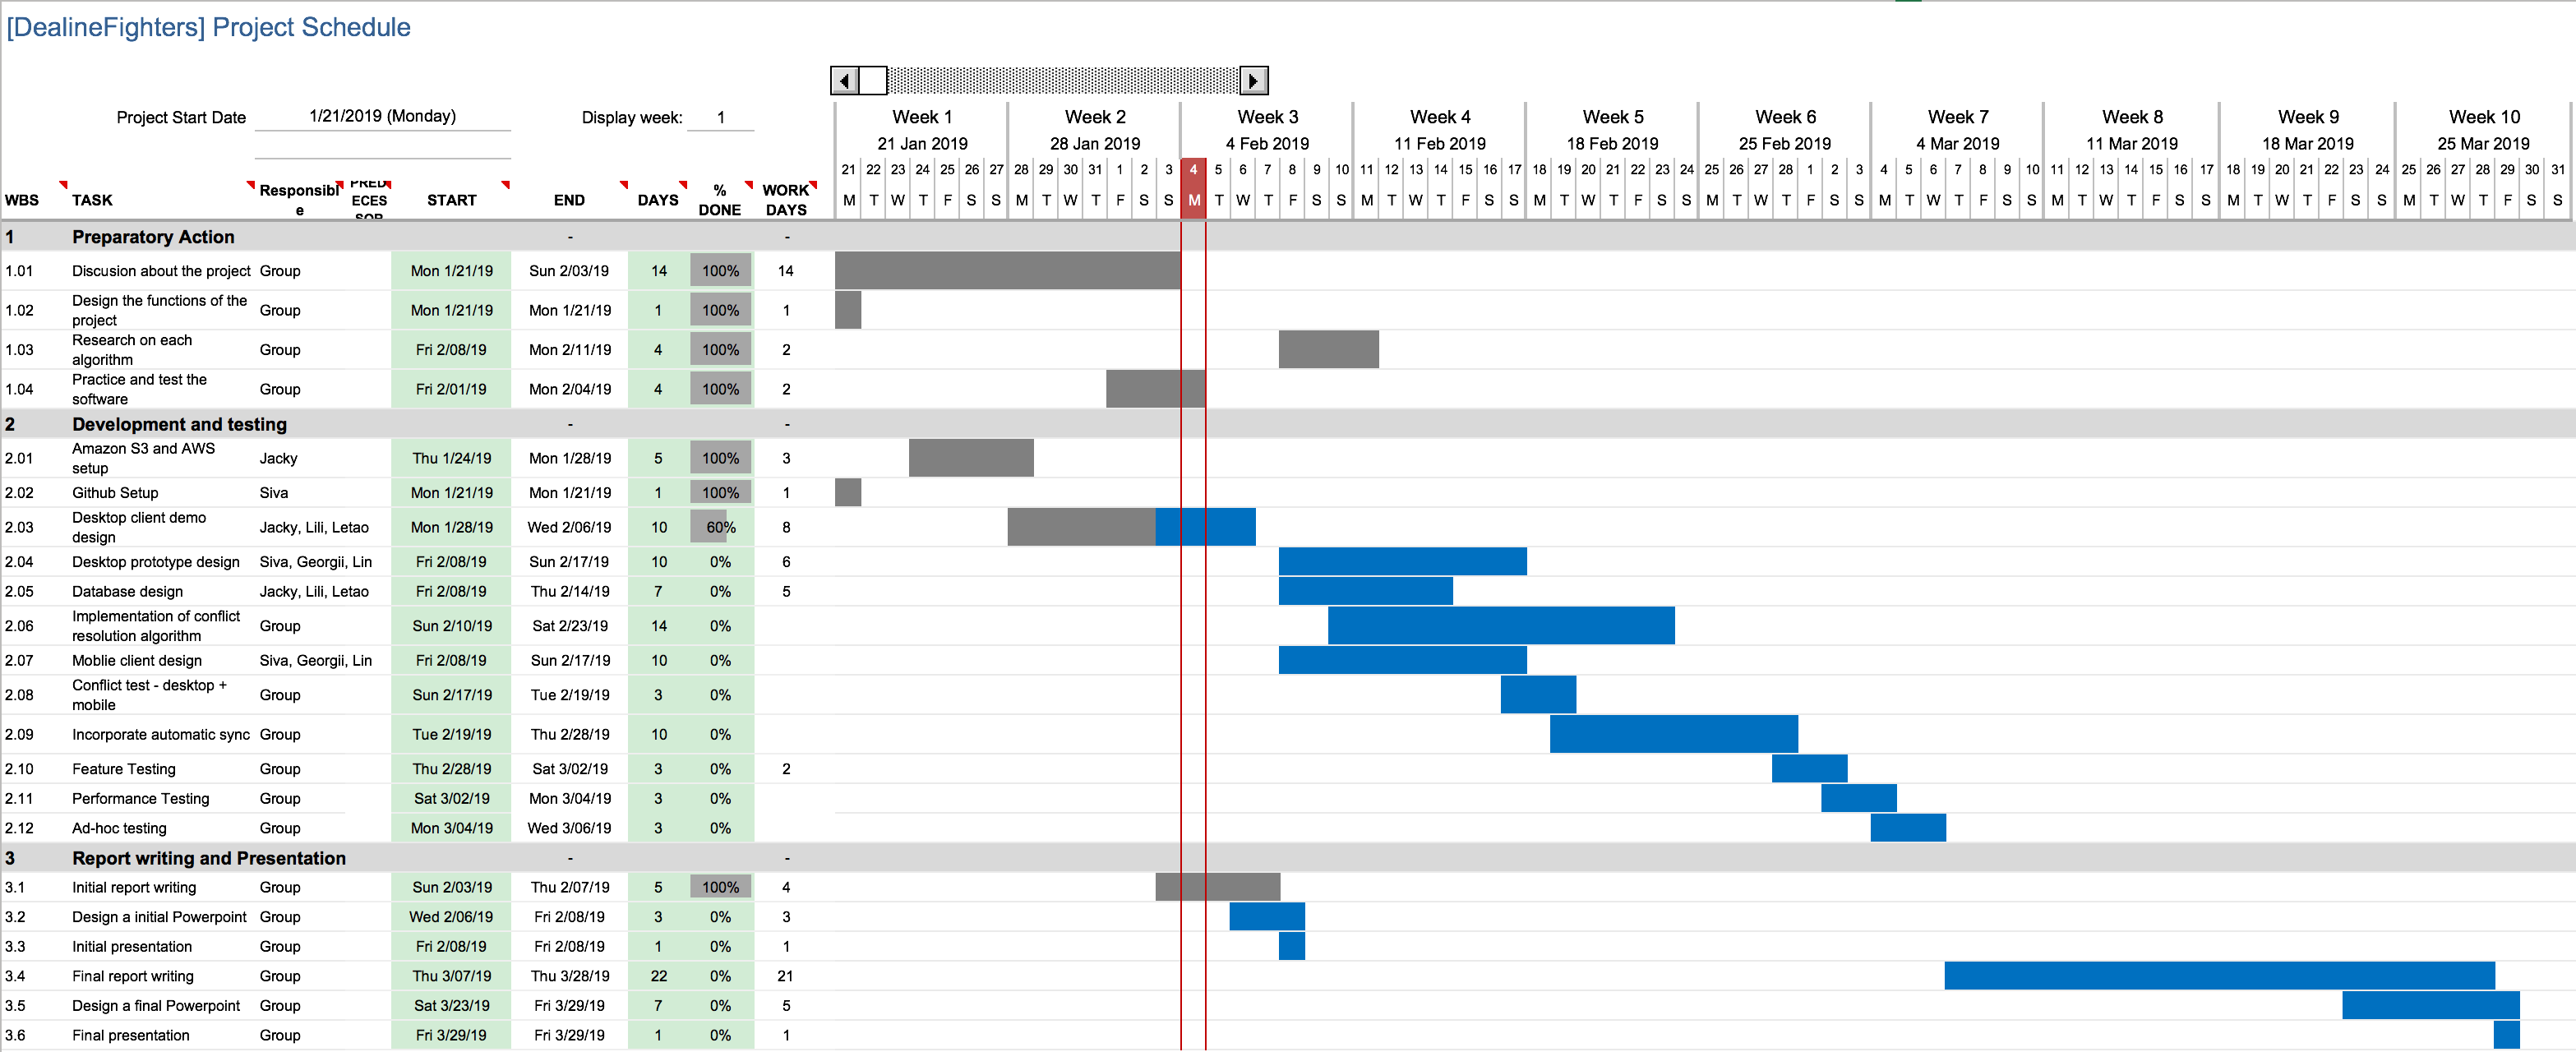
\includegraphics[scale=0.4]{Timeline_Ver_0}
\caption{This is Gantt chart which illustrates the plan of our group within 10 weeks.}
\end{sidewaysfigure}
\end{document}
